% Generated from archived main-run evidence; not an IEEE paper.
% Requires \usepackage{booktabs,graphicx}. Use figure* for wide two-panel figures.
\begin{table*}[t]
\centering
\caption{Main-run descriptive results. Each value is the median of ten runs; Q1 and Q3 are quartiles, not confidence limits. Memory is the median of per-run mean Docker MemUsage.}
\label{tab:performance}
\small
\begin{tabular}{lrrrr}
\toprule
Image & Startup (ms) & Requests/s [Q1, Q3] & Per-run p99 (ms) & Memory (MiB) \\
\midrule
Debian Slim & 501.0 & 280.95 [272.37, 284.15] & 223.5 & 31.28 \\
Alpine & 540.5 & 254.70 [246.69, 262.05] & 250.0 & 29.82 \\
Distroless & 557.0 & 284.07 [277.04, 288.28] & 223.5 & 32.60 \\
\bottomrule
\end{tabular}
\end{table*}

\begin{table*}[t]
\centering
\caption{Docker-reported local size and deduplicated reported findings. Finding identity is (vulnerability ID, package, installed version), not vulnerability ID alone.}
\label{tab:security}
\small
\begin{tabular}{lrrrrr}
\toprule
Image & Size (MB) & OS findings & Application findings & Other language findings & Total \\
\midrule
Debian Slim & 331.68 & 290 & 7 & 51 & 348 \\
Alpine & 234.61 & 73 & 7 & 51 & 131 \\
Distroless & 209.33 & 71 & 7 & 0 & 78 \\
\bottomrule
\end{tabular}
\end{table*}

% Example wide figure:
% \begin{figure*}[t]
% \centering
% 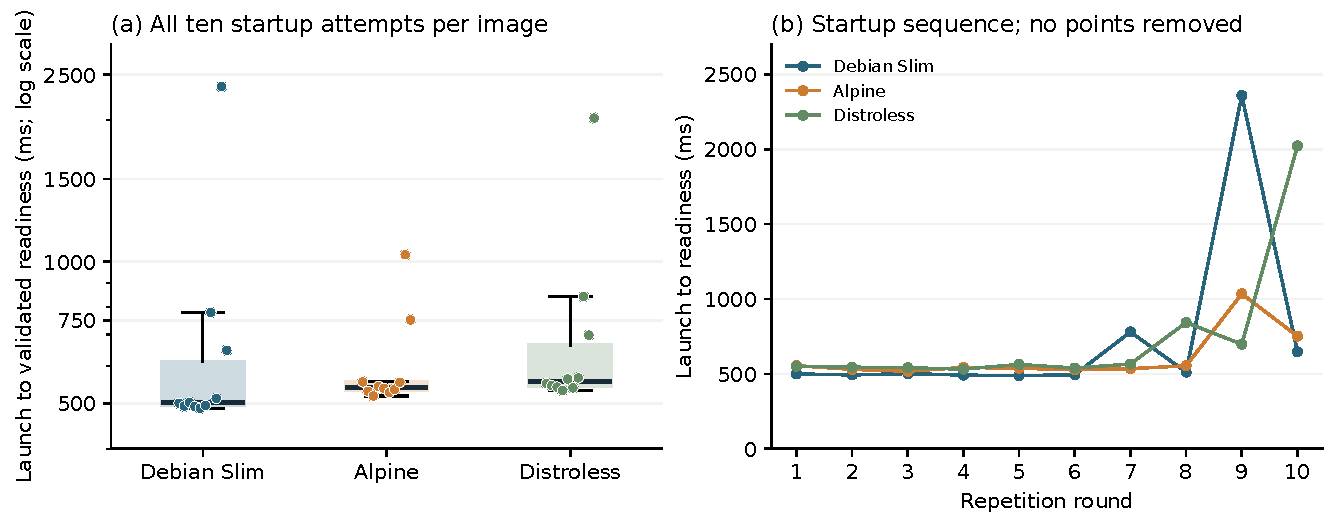
\includegraphics[width=\textwidth]{analysis/figures/03_startup_distribution_and_rounds.pdf}
% \caption{All ten startup attempts per image and startup order by repetition round. No points were removed. The distribution panel uses a logarithmic vertical scale.}
% \label{fig:startup}
% \end{figure*}
